\documentclass[16pt]{article}
\usepackage{graphicx} % Required for inserting images
\usepackage{float}
\floatstyle{plaintop}
\usepackage{geometry}
\usepackage[skip=10pt plus1pt,indent=50pt]{parskip}
\usepackage{setspace}
\usepackage{blindtext}
\usepackage{fancyhdr}
\usepackage[T1]{fontenc}
\usepackage{mathptmx}
\usepackage{hyperref}
\usepackage[table]{xcolor}
\usepackage{multirow}
\usepackage[sorting=none]{biblatex}
\usepackage{lastpage} % used to display we are located in which page 
                      % out of all pages in report
                      
\hypersetup{ % setting options for hyperlinks
    colorlinks=true,    
    linkcolor=black,
    urlcolor=cyan,
    citecolor=black,
}

\onehalfspacing %% set the text spacing the onehalf paragraph

\topmargin 0.1in % giving a margin from the top of page
\headsep 30pt    % giving seperation after the headers

\title{\bf{ Izmir Institute of Technology \\ Computer Engineering Department \\ CENG513 Programming Assignment 1}}
\author{Student Name: Gökay Gülsoy Student No: 270201072}
\date{\today}
\graphicspath{Images/}
\definecolor{myGray}{RGB}{226, 222, 222}

\addbibresource{references.bib}
\begin{document}
\pagecolor{myGray}
\pagestyle{fancy}
% setting the head rule width and footer rule width
\renewcommand{\headrulewidth}{1pt}
\renewcommand{\footrulewidth}{1pt}
\renewcommand{\headruleskip}{2mm}
\renewcommand{\footruleskip}{2mm}

\setlength{\arrayrulewidth}{0.5mm}
\setlength{\tabcolsep}{8pt}
\renewcommand{\arraystretch}{1.5}

\fancyhead{} % clear all header fields
\fancyhead[L]{\bf CENG513 Compiler Design and Construction}
\fancyfoot{} % clear all footer fields
\fancyfoot[L]{\thepage\ of \pageref{LastPage}}
\fancyfoot[C]{\bf Introduction to LLVM}
\fancyfoot[R]{\bf Programming Assignment 1}

\maketitle
\begin{figure}[H]
    \centering
    \includegraphics[scale = 0.45]{Images/iyte_logo.png}
\end{figure}

\newpage
\section*{System Configuration}
   My system configuration for executing the benchmarks is as follows:
    \begin{itemize}
        \item Processor: Intel Core i7-10750H CPU @ 260 GHzX12
        \item Operating System: Ubuntu 22.04.4 LTS
        \item Memory: 16,00 GiB  
        \item GCC Compiler: gcc 11.4.0
        \item Clang Compiler: clang 19.0.0
    \end{itemize}
    
\section*{Building LLVM Test Suite and Running Benchmarks}
   \vspace{5pt}
   \noindent Commands to be executed for building\cite{Getting-Started-with-the-LLVM-System}\cite{What-is-LLVM}\cite{Installing-LLVM} and running benchmarks is as follows:
    \begin{enumerate}
        \item Command to check for llvm-lit version: /home/gokay/llvm-project/build/bin/llvm-lit --version
        \item Command to clone the llvm-test-suite: git clone \url{https://github.com/llvm/llvm-test-suite.git}
        \item Command to create build directory: mkdir test-suite-build
        \item Command to change directory to build directory: cd test-suite-build
        \item Command to write build files into build directory: cmake -D\verb|_|CMAKE\verb|_|COMPILER=\verb|~| llvm-project/build/bin/clang -C ../cmake/caches/O3.cmake ..
        \item Command to make the llvm-test-suite from test-suite-build directory: make
        \item Command to run the tests: llvm-lit -v -j 8 -o results.json
    \end{enumerate}
    

    \noindent
    I run the 7th command three times for clang and three times for the gcc compiler to obtain execution time benchmarks from Multisource directory. Inorder to build llvm-test-suite with gcc, 5th command can be configured as follows and llvm-test-suite can be rebuild after that with make\cite{test-suite}:
    \begin{itemize}
        \item cmake -D\verb|_|CMAKE\verb|_|COMPILER=/usr/bin/gcc -C ../cmake/caches/O3.cmake ..
    \end{itemize}
    \vspace{5pt}
    Following are the applications that I have chosen for running benchmarks:
    \begin{enumerate}
        \item MultiSource/Benchmarks/llubenchmark/llu
        \item MultiSource/Benchmarks/7zip/7zip-benchmark
        \item MultiSource/Benchmarks/Reductions-flt/Reductions-flt
        \item MultiSource/Benchmarks/NPB-serial/is/is
        \item MultiSource/Benchmarks/Bullet /bullet
    \end{enumerate}

    \vspace{5pt}
    \noindent
    Execution time statistic that I have obtained are as follows:

    \noindent
    \begin{table}[h!]
    \rowcolors{1}{gray}{lightgray}
    \centering
    \begin{tabular}{ |p{2.5cm}|p{2.5cm}|p{2.5cm}|p{2.5cm}|p{2.5cm}| }
    \hline
    \rowcolor{lightgray}\multicolumn{5}{|c|}{Benchmark Results GCC} \\
    \hline
    \rowcolor{green!80!yellow!50}
    llu & 7zip-benchmark & Reduction-flt & is & bullet \\
    \hline
    15.5266s & 9.2371s & 5.8437s  & 5.7246s  & 4.2390s  \\
    11.6043s & 8.6455s & 5.2043s  & 5.3806s  & 3.4759s \\
    9.9513s  & 8.5745s &  5.1098s & 5.8200s & 2.8970s \\
    \hline
    \end{tabular}
    \caption{Execution time statistics for gcc}
    \label{GCC execution statistics}
    \end{table}

    \noindent
    Table \ref{GCC execution statistics} shows the execution time statistics for the applications that I have tested with gcc. Following table shows execution 
    time statistic for clang:

    \noindent
    \rowcolors{1}{gray}{lightgray}
    \begin{table}[h!]
    \centering
    \begin{tabular}{ |p{2.5cm}|p{2.5cm}|p{2.5cm}|p{2.5cm}|p{2.5cm}| }
    \hline
    \rowcolor{lightgray}\multicolumn{5}{|c|}{Benchmark Results Clang} \\
    \hline
    \rowcolor{green!80!yellow!50}
    llu & 7zip-benchmark & Reduction-flt & is & bullet \\
    \hline
    7.8791s & 7.3820s & 3.8842s & 3.2795s & 4.4335s  \\
    8.5101s & 11.8736s & 3.9758s & 5.3109s   & 5.0810s \\
    10.9066s  & 9.4378s &  8.9971s & 6.2024s & 7.0257s \\
    \hline
    \end{tabular}
    \caption{Execution time statistics for clang}
    \label{Clang execution statistics}
    \end{table}

    \noindent
    Average Execution time statistics for the benchmark applications which are given in table \ref{GCC execution statistics} with gcc are indicated in table \ref{GCC average execution statistics} and average execution time statistics for the clang are indicated in table \ref{Clang average execution statistics}:

    \clearpage %% advance to new page
    
    \noindent
    \rowcolors{1}{gray}{lightgray}
    \begin{table}
    \centering
    \begin{tabular}{ |p{2.5cm}|p{2.5cm}|p{2.5cm}|p{2.5cm}|p{2.5cm}| }
    \hline
    \rowcolor{lightgray}\multicolumn{5}{|c|}{Average Benchmark Results GCC} \\
    \hline
    \rowcolor{green!80!yellow!50}
    llu & 7zip-benchmark & Reduction-flt & is & bullet \\
    \hline
     12.3607s & 8.8190s & 5.3859s & 5.6417s & 3.5373s  \\
    \hline
    \end{tabular}
    \caption{Average execution time statistics for gcc}
    \label{GCC average execution statistics}
    \end{table}

    \noindent
    \rowcolors{1}{gray}{lightgray}
    \begin{table}
    \centering
    \begin{tabular}{ |p{2.5cm}|p{2.5cm}|p{2.5cm}|p{2.5cm}|p{2.5cm}| }
    \hline
    \rowcolor{lightgray}\multicolumn{5}{|c|}{Average Benchmark Results Clang} \\
    \hline
    \rowcolor{green!80!yellow!50}
    llu & 7zip-benchmark & Reduction-flt & is & bullet \\
    \hline
    9.0986s & 9.5644s & 5.6190s & 4.9309s & 5.5134s  \\
    \hline
    \end{tabular}
    \caption{Average execution time statistics for clang}
    \label{Clang average execution statistics}
    \end{table}
    \noindent
    Visualization of benchmark results and their comparison in gcc and clang are as given in the following figure:
    \begin{figure}[h!]
        \centering
        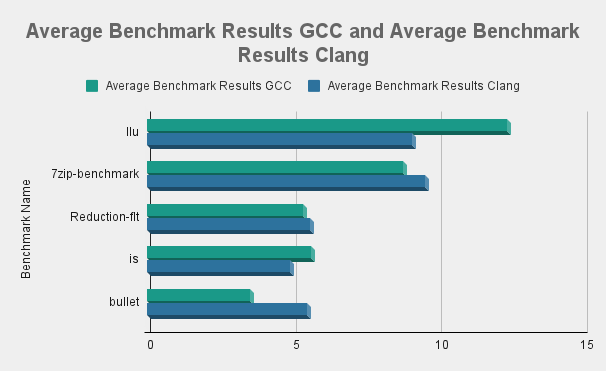
\includegraphics[width=0.96\linewidth]{Average Benchmark Results GCC and Average Benchmark Results Clang.png}
        \caption{GCC and Clang benchmark execution time comparison}
        \label{fig1: GCC and Clang becnhmark time comparison}
    \end{figure}

    As we can observe from the execution of benchmarks give in the figure \ref{fig1: GCC and Clang becnhmark time comparison} for the applications that I have chosen, gcc has shorter execution time on average for three of the benchmarks and clang has shorter execution time on average for two of the benchmarks.
    % all paragraphs apart from the first paragraph inside
    % sections will be indented by the amount given by parskip 
    % package which is 40 pt for now
    \printbibliography

\end{document}
